\section{David Wineland}

\begin{frame}[t]{David Wineland: In a nutshell}
  \portraitpic{wineland.jpg}
  \vspace{3cm}
  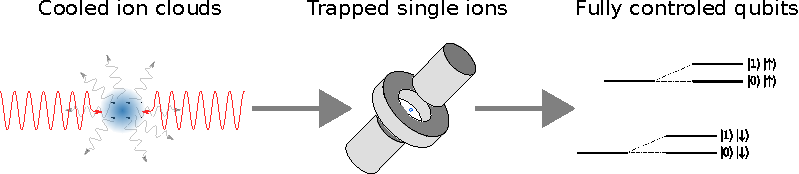
\includegraphics[width=\textwidth]{dw_nutshell.pdf}
\end{frame}

\begin{frame}[t]{David Wineland: Early life}
  \portraitpic{wineland.jpg}
  \visible<3>{
    \textpos{\linewidth}{0cm}{3cm}{\begin{quote}``I knew I was destined to go to
    college and I always kept up my grades to be able to do that''\end{quote}}
  }
  \visible<6>{
    \textpos{\linewidth}{0cm}{3cm}{\begin{quote}``Because I respected my
        classical mechanics teacher so
    much, I asked him about places to apply for graduate school. He recommended
  Harvard, so I applied there.''\end{quote}}
  }
  \begin{minipage}[t][4.5cm][t]{\textwidth-1.5cm}
    \begin{itemize}
      \item<1-> Born near Milwaukee, Wisconsin
      \item<2-> Parents moved to Sacramento, California
      \item<4-> Math Major at University of California, Davis
      \item<5-> Transfer to Berkeley as Physics Major
    \end{itemize}  
  \end{minipage}

  \begin{minipage}[t][0.2\textheight][t]{\textwidth}
    \begin{chronology}[10]{1940}{2016}{\textwidth}{5cm}
      \visible<1>{\event{1944}{24.02.1944}}
      \visible<2>{\event{1947}{'47}}
      \visible<4>{\event{1961}{'61}}
      \visible<5>{\event[1962]{1965}{'62 -- '65}}
    \end{chronology}
  \end{minipage}
\end{frame}

\begin{frame}[t]{David Wineland: Scientific Carreer}
  \portraitpic{wineland.jpg}
  \visible<1>{
    \picpos{6.5cm}{1cm}{1.5cm}{norman_ramsey_group_np.jpg}
    \source{Nobel lecture D. Wineland}
  }
  \begin{minipage}[t][4.5cm][t]{\textwidth-1.5cm}
    \begin{itemize}
      \item Master and PhD at Norman Ramseys group in Harvard
      \item<2> Spectroscopy of hyperfine levels of Deuterium
    \end{itemize}  
  \end{minipage}
  \begin{minipage}[t][0.2\textheight][t]{\textwidth}
    \begin{chronology}[10]{1940}{2016}{\textwidth}{5cm}
      \event[1965]{1970}{'65 -- '70}
    \end{chronology}
  \end{minipage}
\end{frame}

\begin{frame}[t]{David Wineland: Scientific Carreer}
  \portraitpic{wineland.jpg}
  \visible<1>{
    \picpos{3cm}{1cm}{1.5cm}{hans_dehmelt_np.jpg}
    \source{{wikimedia, inkscape}}
  }
  \visible<4->{\source{{PhysRevLett73, inkscape}}}
  \visible<2>{
    \picpos{8cm}{1cm}{2cm}{monoelectron_title.jpg}
    \source{PhysRevLett73}
  }
  \visible<3>{
    \picpos{8cm}{0.5cm}{2cm}{dw_penning_trap.pdf}
  }
  \visible<4->{
    \picpos{9cm}{1cm}{2.5cm}{dw_monoelectron_plot.pdf}
  }
  \visible<5>{
    \picpos{9cm}{1cm}{2.5cm}{dw_monoelectron_plot1.pdf}
  }
  \visible<6>{
    \picpos{9cm}{1cm}{2.5cm}{dw_monoelectron_plot2.pdf}
  }
  \visible<7>{
    \picpos{9cm}{1cm}{2.5cm}{dw_monoelectron_plot3.pdf}
  }
  \begin{minipage}[t][4.5cm][t]{\textwidth-1.5cm}
    \begin{itemize}
      \item Postdoc in Hans Dehmelts group in Washington
      \item<2-> Trapping single electrons in a Penning trap
    \end{itemize}  
  \end{minipage}
  \begin{minipage}[t][0.2\textheight][t]{\textwidth}
    \visible<1-2>{
      \begin{chronology}[10]{1940}{2016}{\textwidth}{5cm}
        \visible<1>{\event[1970]{1975}{'70 -- '75}}
        \visible<2>{\event{1973}{'73}}
      \end{chronology}
    }
  \end{minipage}
\end{frame}

\begin{frame}[t, noframenumbering]{David Wineland: Scientific Carreer}
  \portraitpic{wineland.jpg}
  \visible<1->{
    \picpos{7cm}{1cm}{2.5cm}{doppler_cooling.pdf}
  }
  \begin{minipage}[t][4.5cm][t]{\textwidth-1.5cm} %TODO Citation of paper
    \begin{itemize}
      \item Postdoc in Hans Dehmelts group in Washington
      \item Idea of laser cooling of ions (Doppler cooling)
    \end{itemize}  
  \end{minipage}
  \begin{minipage}[t][0.2\textheight][t]{\textwidth}
    \begin{chronology}[10]{1940}{2016}{\textwidth}{5cm}
      \visible<>{\event[1970]{1975}{'70 -- '75}}
      \visible<1>{\event{1975}{'75}}
    \end{chronology}
  \end{minipage}
\end{frame}

\begin{frame}[t]{David Wineland: Scientific Carreer}
  \portraitpic{wineland.jpg}
  \visible<2->{
    \picpos{4.5cm}{1cm}{2.1cm}{dw_cs_clock.jpg}
    \source{Nobel lecture D. Wineland}
  }
  \begin{minipage}[t][4.5cm][t]{\textwidth-1.5cm} 
    \begin{itemize}
      \item Position at the time and frequency division of the national bureau
        of standards (NBS, later NIST)

      \item In charge of setting up a working Cesium clock
    \end{itemize}  
  \end{minipage}
  \begin{minipage}[t][0.2\textheight][t]{\textwidth}
    \begin{chronology}[10]{1940}{2016}{\textwidth}{5cm}
      \visible<1>{\event[1975]{1977}{'75 -- '77}}
    \end{chronology}
  \end{minipage}
\end{frame}

\begin{frame}[t]{David Wineland: Scientific Carreer}
  \portraitpic{wineland.jpg}
  \visible<1>{
    \picpos{6cm}{1cm}{1.5cm}{dw_group_79.jpg}
    \source{Nobel lecture D. Wineland}
  }
  
  \visible<3>{
    \picpos{9cm}{1cm}{2.5cm}{dw_doppler_cooling_title_full.jpg}
  }

  \visible<4-5>{
    \picpos{5.5cm}{0.5cm}{3cm}{dw_laser_cooling_ions_setup.pdf}
  }

  \visible<5>{
    \picpos{5.5cm}{6cm}{3.5cm}{dw_laser_cooling_ions_plot.pdf}
    \source{{Nobel lecture D. Wineland, inkscape}}
  }

  \visible<6>{
    \picpos{9cm}{1cm}{2.5cm}{dw_doppler_cooling_title.jpg}
  }
  
  \visible<6>{
    \picpos{9cm}{1cm}{4.8cm}{dehmelt_toschek_cooling_title.jpg}
  }
   
  \visible<2>{
    \textpos{\linewidth}{0cm}{3cm}{\begin{quote}``I knew that we had competition
    because I was aware that Dehmelt had taken a sabbatical to work in Peter
Toschek's lab in Heidelberg, with the same goal of demonstrating cooling.''\end{quote}}
  }
  \begin{minipage}[t][4.5cm][t]{\textwidth-1.5cm}
    \begin{itemize}
      \item<1-> Own group at NBS to research trapped ions and lasers
      \item<2-> Taking up the earlier idea of Doppler cooling
    \end{itemize}  
  \end{minipage}
  \begin{minipage}[t][0.2\textheight][t]{\textwidth}
    \visible<1>{
      \begin{chronology}[10]{1940}{2016}{\textwidth}{5cm}
        \event[1977]{2016}{'77 -- '16 }
      \end{chronology}
    }
  \end{minipage}
\end{frame}

\begin{frame}[c]
  \begin{center}
      \Large Trapped single electrons and cooled down ion clouds, what is next?  
  \end{center}
\end{frame}

\begin{frame}[t]{David Wineland: Research}
  \portraitpic{wineland.jpg}
  \visible<1,5>{
    \picpos{9cm}{.7cm}{1.7cm}{dw_single_mg_title.pdf}
    \source{PhysLettA81}
  }
  \visible<2-4>{
    \picpos{8cm}{1cm}{1.5cm}{dw_single_mg_plot.pdf}
    \source{PhysLettA81}
  }
  \visible<3>{\picpos{8cm}{1cm}{1.5cm}{dw_single_mg_plot1.pdf}}
  \visible<4>{\picpos{8cm}{1cm}{1.5cm}{dw_single_mg_plot2.pdf}}
  \visible<5>{\picpos{9cm}{.7cm}{4.1cm}{dehmelt_mono_ion_title.pdf}}

  \begin{minipage}[t][4.5cm][t]{\textwidth-1.5cm}
    \begin{itemize}
      \item Trapping of single ions
    \end{itemize}  
  \end{minipage}
  \begin{minipage}[t][0.2\textheight][t]{\textwidth}
    \visible<1>{
      \begin{chronology}[10]{1940}{2016}{\textwidth}{5cm}
        \event{1981}{'81 }
        \visible<>{\event{1999}{'99 -- '99}} %this will never be visible, just
      \end{chronology}
    }
  \end{minipage}
\end{frame}

\begin{frame}[t]{David Wineland: Ion Quantum Jumps}
  \portraitpic{wineland.jpg}

  \visible<1>{
    \picpos{8cm}{0.5cm}{1.9cm}{DW_quantum_jumps_title.pdf}
  }
  \visible<2-4>{\source{Nobel lecture D. Wineland, inkscape}}
  \visible<2>{\picpos{7.5cm}{0cm}{1.9cm}{dw_quantum_jumps_scheme0.pdf}}
  \visible<3>{\picpos{7.5cm}{0cm}{1.9cm}{dw_quantum_jumps_scheme1.pdf}}
  \visible<4>{\picpos{7.5cm}{0cm}{1.9cm}{dw_quantum_jumps_scheme2.pdf}}
  \visible<4>{\textpos{5cm}{7.5cm}{4.5cm}{\small fluorescence only when ion occupies
    ground state}}
  \visible<5>{\picpos{7.5cm}{0cm}{1.9cm}{dw_quantum_jumps_scheme_level.pdf}\source{PhysRevLett86}}
  
  \visible<5>{
    \picpos{7cm}{2.8cm}{3cm}{DW_quantum_jumps_results.pdf}
    \textpos{6cm}{3cm}{5.5cm}{\small $\rightarrow$ quantum jumps between ground
    and excited state}
  }
  \begin{minipage}[t][4.5cm][t]{\textwidth-1.5cm}
    \begin{itemize}
      \item Quantum jumps of an ions electron shell
    \end{itemize}  
  \end{minipage}
  \begin{minipage}[t][0.2\textheight][t]{\textwidth}
    \visible<1>{
      \begin{chronology}[10]{1940}{2016}{\textwidth}{5cm}
        \event{1986}{'86 }
        \visible<>{\event{1999}{'99 -- '99}} %this will never be visible, just
      \end{chronology}
    }
  \end{minipage}
\end{frame}

\begin{frame}[t]{David Wineland: Research}
  \portraitpic{wineland.jpg}
  \visible<1>{
    \picpos{8cm}{0.5cm}{1.9cm}{dw_recoilless_single_ion_title.pdf}
  }

  %\visible<2>{
  %  \picpos{\textwidth}{0cm}{1.9cm}{dw_quantized_motion_plot.pdf}
  %}
  \begin{minipage}[t][4.5cm][t]{\textwidth-1.5cm}
    \begin{itemize}
      \item Quantized motional states of the ion in the trap can be resolved
        with a tunable laser
    \end{itemize}  
  \end{minipage}
  \begin{minipage}[t][0.2\textheight][t]{\textwidth}
    \visible<1>{
      \begin{chronology}[10]{1940}{2016}{\textwidth}{5cm}
        \event{1987}{'87 }
        \visible<>{\event{1999}{'99 -- '99}} %this will never be visible, just
      \end{chronology}
    }
  \end{minipage}
\end{frame}

\begin{frame}[t]{David Wineland: Sideband Cooling}
  \portraitpic{wineland.jpg}
  \source{{Nobel lecture D. Wineland, inkscape}}
  \visible<1>{
    \picpos{8cm}{0.5cm}{1.9cm}{DW_zero_point_energy_title.pdf}
  }
  \visible<2>{
    \picpos{\textwidth}{0cm}{1.9cm}{sideband_cooling_scheme_2_0.pdf}
  }
  \visible<3>{
    \picpos{\textwidth}{0cm}{1.9cm}{sideband_cooling_scheme_3.pdf}
  }
  \visible<4>{
    \picpos{\textwidth}{0cm}{1.9cm}{sideband_cooling_scheme_4.pdf}
  }
  \visible<5>{
    \picpos{\textwidth}{0cm}{1.9cm}{sideband_cooling_scheme_5.pdf}
  }
  \visible<6>{
    \picpos{\textwidth}{0cm}{1.9cm}{sideband_cooling_scheme_6.pdf}
  }
  \visible<7>{
    \picpos{\textwidth}{0cm}{1.9cm}{sideband_cooling_scheme_7.pdf}
    \textpos{4cm}{7.5cm}{6cm}{\small $\rightarrow$ Atom cooled to motional ground state}
  }
  \visible<2->{
    \picpos{\textwidth}{0cm}{1.9cm}{sideband_cooling_scheme_states.pdf}
  }
  \begin{minipage}[t][4.5cm][t]{\textwidth-1.5cm}
    \begin{itemize}
      \item Resolved sideband cooling to motional ground state
    \end{itemize}  
  \end{minipage}
  \begin{minipage}[t][0.2\textheight][t]{\textwidth}
    \visible<1>{
      \begin{chronology}[10]{1940}{2016}{\textwidth}{5cm}
      \visible<>{\event{1999}{'99 -- '99}} %this will never be visible, just
        \event{1989}{'89}
      \end{chronology}
    }
  \end{minipage}
\end{frame}


\begin{frame}[t]{David Wineland: Quantum Logic Gate}
  \portraitpic{wineland.jpg}
  \visible<1>{\picpos{9cm}{0.5cm}{1.5cm}{DW_cnot_gate_title.pdf}}
  \visible<2->{\picpos{5cm}{0.8cm}{2.5cm}{qubits.pdf}}
  \visible<2>{\textpos{5cm}{6.4cm}{3.5cm}{internal qubit
    $\begin{cases}\ket{\uparrow} \\ \ket{\downarrow}\end{cases}$}}
  \visible<2>{\textpos{5cm}{7cm}{5cm}{trap qubit
    $\begin{cases}\ket{0} \\ \ket{1}\end{cases}$}}
  \visible<3-5>{\textpos{6cm}{5.4cm}{3.8cm}{\begin{itemize}\item 4 possible pure
      states \item superposition states can be engineered by laser
pulses \item<5> basic logic operations possible\end{itemize}}}
  \visible<4>{\textpos{8cm}{0.8cm}{6cm}{$\ket{0}\ket{\downarrow}
  \xrightarrow[\text{blue sideband}]{\hspace{0.5cm}\pi/2\text{-pulse on}\hspace{0.5cm}}
  \frac{1}{\sqrt{2}}\left( \ket{0}\ket{\downarrow} + \ket{1}\ket{\uparrow}\right)$}}

  \visible<4>{\picpos{5cm}{0.8cm}{2.5cm}{qubits_arrow.pdf}}
  \begin{minipage}[t][4.5cm][t]{\textwidth-1.7cm}
    \begin{itemize}
      \item Use of trapped ion to store and manipulate two qubits
    \end{itemize}  
  \end{minipage}
  \begin{minipage}[t][0.2\textheight][t]{\textwidth}
    \visible<1>{
      \begin{chronology}[10]{1940}{2016}{\textwidth}{5cm}
        \event{1996}{'95 }
        \visible<>{\event{1999}{'99 -- '99}} %this will never be visible, just
      \end{chronology}
    }
  \end{minipage}
\end{frame}

\begin{frame}[t]{David Wineland: Quantum Logic Gate}
  \portraitpic{wineland.jpg}
  \visible<2->{\picpos{4cm}{0.8cm}{2.8cm}{controled_not.pdf}}
  \visible<3->{\picpos{6cm}{5.2cm}{2.8cm}{DW_cnot_gate_truthtable.pdf}
  \source{PhysRevLett96}}

  \begin{minipage}[t][4.5cm][t]{\textwidth-1.7cm}
    \begin{itemize}
      \item Controled NOT gate (CNOT): flip target qubit ($\ket{\uparrow}$ or
        $\ket{\downarrow}$) only if control qubit ($\ket{0}$ or $\ket{1}$) is $\ket{1}$
    \end{itemize}  
  \end{minipage}
  \begin{minipage}[t][0.2\textheight][t]{\textwidth}
    \visible<>{
      \begin{chronology}[10]{1940}{2016}{\textwidth}{5cm}
        %\event{1996}{'95 }
        \visible<>{\event{1999}{'99 -- '99}} %this will never be visible, just
      \end{chronology}
    }
  \end{minipage}
\end{frame}
